%%%%
%%%% Main Matter
%%%%

\addstarredpart{Part Zero}

\cleardoublepage
\chapter*{Table des matières}
\parttoc

%\addcontentsline{toc}{xpart}{}
%\addcontentsline{tdm}{section}{Tututututu}

\chapter[Introduction]{Introduction}


\section{Block ciphers}

A \emph{block cipher} is a family of injective mappings over finite domains and co-domains, indexed by a finite set of \emph{keys}. This very broad definition will
in fact always be specialized, taking domains and co-domains of identical sizes, and all parameters living in the binary world. Hence, a block cipher
is a mapping $\E : \{0,1\}^\kappa \times \{0,1\}^n \rightarrow \{0,1\}^n$ such that for all $k \in \{0,1\}^\kappa$, $\E(k,\cdot)$ is a permutation.
We call $\kappa$ the \emph{key size} and $n$ the \emph{block size} of $\E$. Typical parameter sizes are $\kappa \in \{64, 80, 128, 192, 256\}$ (though
64 and 80-bit keys are now considered to be too short to provide adequate security) and $n \in \{64, 128, 256\}$.
We usually require $\E$ and its inverse $\E^{-1}$ to be efficiently computable (depending on the intended application, it may be enough for only
one of these to be efficient).

The most immediate purpose of block ciphers is to provide confidentiality of communications. Two parties $A$ and $B$ who share a key $k$\footnote{We
completely ignore the problem of obtaining such a shared key.} for the same
block cipher are able to send encrypted messages $c \defas \E(k,p)$, $c' \defas \E(k,p')$, etc. The non-key input to $\E$ is generally called
the \emph{plaintext}, and the output of $\E$ is called the \emph{ciphertext}.

If $\E$ is such that the permutations $\E(k,\cdot)$ are hard to invert when $k$ is unknown, $A$ and $B$ may suppose that a secure channel of communication
between them consists in injecting their messages to strings $m_0||m_1||\ldots||m_\ell$ of sizes multiple of $n$ and sending encrypted messages
$\E(k,m_0)||\E(k,m_1)||\ldots||\E(k,m_\ell)$. There are two major problems with this scheme, however, regardless of the security of the block
cipher: 1) The scheme is not \emph{randomised}, \ie encrypting the same plaintext twice always results in the same ciphertext. An eavesdropper
(a ``passive adversary'') on the channel between $A$ and $B$ can thus detect when identical message blocks have been sent. 2) The
communication is not authenticated. An active adversary on the channel may delete or modify some of the blocks of a message, append to a message
some blocks from a previous message, or add randomly generated blocks. All of this can be done without $A$ and $B$ noticing that someone
is maliciously tampering with the channel.

Problems such as the ones above are solved by designing secure \emph{modes of operation}. We do not study this topic in this thesis, but
we mention some elements related to modes in \autoref{sec:bc_modes}. But first, we make the intuition behind the evaluation of the security
of block ciphers themselves more explicit in \autoref{sec:bc_sec}.

\subsection{Security of block ciphers}

We keep this section relatively informal. Our goal is to be able to specify what it means for $\E$ to be a good block cipher from
a practical point of view. Yet, we start by defining the useful notion of \emph{ideal block cipher}.

\begin{defi}[Ideal block cipher]
An \emph{ideal block cipher} $\E$ is a mapping $\{0,1\}^\kappa \times \{0,1\}^n \rightarrow \{0,1\}^n$ s.t. all the permutations
$\E(k,\cdot)$ are drawn independently and uniformly at random among the permutations of $\{0,1\}^n$.
\end{defi}

This definition intuitively corresponds to the best we can achieve from the definition of a block cipher. For small values of $n$
(\eg up to $20 \sim 32$ depending on the desired performance), one can implement ideal block ciphers by using an appropriate
shuffling algorithm (such as the one variously attributed to Fisher, Yates, Knuth, etc.~\cite{uniform_shuffle}, which we will
call ``FYK''). As this method
requires $\bigo(2^n)$ setup time and memory per key, it is obviously impractical for cryptographically common block sizes of $n \geq 64$.
Even for small values of $n$, running the FYK shuffle requires a considerable amount of randomness parameterized by the keys, which
is not something trivial to fulfill. All of this leads to the fact that we are forced most of the time to use ``approximations'' of
ideal block ciphers. A useful (mostly theoretical) way of quantifying the security of a specific block cipher is to measure ``how far'' it
is from being ideal. Informally, this is done by upper-bounding the \emph{advantage} (over a random answer) that any adversary
(with some bounded resources)
has of distinguishing whether he is given black-box access to a randomly-drawn permutation or to an instance of the block cipher
with a randomly chosen (unknown) key. This statement can be made more precise in the form of the following definition
(similar to the one that can be found \eg in \cite{DBLP:journals/jcss/BellareKR00}):

\begin{defi}[Pseudo-random permutations (PRP)]
We consider a block cipher $\E$ of key size $\kappa$ and block size $n$.
We write $\Pi_{2^n}$ for the set of permutations on binary strings of length $n$; $x \overset{\$}{\leftarrow} \mathcal{S}$
the action of drawing $x$ uniformly at random among elements of the set $\mathcal{S}$; $\mathcal{A}^{f}$ an algorithm with
oracle (black-box) access to the function $f$ and which outputs a single bit.
Then we define the \emph{PRP advantage} of $\mathcal{A}$ over $\E$, written $\Adv^{\text{PRP}}_{\E}(\mathcal{A})$ as:
\[
\Adv^{\text{PRP}}_{\E}(\mathcal{A}) = |\Pr[\mathcal{A}^f = 1~|~f \overset{\$}{\leftarrow} \Pi_{2^n}] - \Pr[\mathcal{A}^f = 1~|~f \defas \E(k,\cdot), k \overset{\$}{\leftarrow} \{0,1\}^\kappa]|.
\]
The \emph{PRP security} of $\E$ w.r.t. the \emph{data complexity} $q$ and \emph{time complexity} $t$ is:
\[
\Adv^{\text{PRP}}_{\E}(q,t) \defas \max_{\mathcal{A}\,\in\,\text{Alg}^{f\backslash q, \E\backslash t}} \{\Adv^{\text{PRP}}_{\E}(\mathcal{A})\}.
\]
Here, $\text{Alg}^{f\backslash q, \E\backslash t}$ is the set of all algorithms $\mathcal{A}$ with oracle access to $f$ that perform at most $q$ oracle accesses
and which run in time $\bigo(t)$, with the time unit being the time necessary to compute $\E$ once.
\end{defi}
There exists a related notion of \emph{strong pseudo-random permutation} (SPRP) where one considers algorithms given oracle access both to $f$ and its inverse.

\medskip

\autoref{def:prp} is quite useful in some contexts, for instance to prove that a construction using a block cipher is not significantly less secure than the latter. This is
typically done by defining an advantage function similar to PRP security for the higher-level construction (this being for instance CBC-MAC in the case of \cite{DBLP:journals/jcss/BellareKR00}) and by showing that
it is not more than the PRP security of the block cipher plus some (reasonably small) extra terms.

However, this definition is not constructive, in the sense that it does not provide any (efficient)
way of computing the PRP security of a block cipher in general (some results do exist for specific block cipher constructions (usually modulo access to a lower-level primitive such as a
``random permutation'') such as the one due to Even and Mansour~\cite{EM}, which we will see again in \autoref{chap:emrka}).
A major topic in symmetric cryptography is to analyse explicit block ciphers in order to assess their concrete security against attacks. In the language of \autoref{def:prp}, this
consists in finding algorithms for which $q$, $t$ and the PRP advantage is known. Any such attack on a block cipher $\E$ allows to lower-bound its PRP-security at a given point.
In reality, though, the world of block cipher cryptanalysis is more nuanced than what \autoref{def:prp} may lead us to believe; practically important characteristics of an attack
are also its memory complexity, distinguishing between its online and offline time complexity, whether it applies equally well to all keys or if it is only successful
for some ``weak'' subset thereof, whether it also recovers $k$ when $f$ was instantiated from $\E$, or an algorithm equivalent to $\E(k,\cdot)$, etc. We devote the remainder of this
section to sketching some typical elements of attacks on block ciphers.

\subsection{Distinguishers and attacks}
The core of many concrete attacks on block ciphers is made of \emph{distinguishers}, which can be defined as algorithms using reasonable resources which have a non-negligible advantage according to \autoref{def:prp}.
There is no easy answer as to what ``reasonable'' and ``non-negligible'' should mean in the context of actual cryptanalysis, as the key and block size of a specific cipher are fixed values. While some ciphers or potential distinguishers
may be parameterized in a way that helps to make the definition meaningful, this does not have to be the case. Sometimes, one is easily convinced by the performance of an algorithm so that there is
consensus that it can be called a distinguisher (\eg distinguishing $\E$ of key and block size $2^{128}$ with $q = 2$, $t = 2^{20}$, probability $\approx 1$), while some other times the picture is much less clear
(\eg $q = t =  2^{120}$ and probability $\approx 1$). We will ignore this issue altogether and assume that all the attacks of this chapter are consensual.

\subsubsection{Classes of distinguishers for block ciphers}

We now briefly describe two examples of types of distinguishers, which exploit ``non-ideal'' behaviours of different nature.

\bigskip

We start with \emph{differential distinguishers}, which are part of the broader class of \emph{statistical} distinguishers.
The basic idea of the latter is to define an event which has a different probability distribution for the target (the block cipher $\E$)
than for a random permutation drawn from $\Pi_{2^n}$. Running the distinguisher then consists in collecting a certain number of samples (obtained through
the oracle) and deciding from which distribution
%(the one entailed by $\E$ or the one entailed by a random permutation)
those are the
most likely to have been drawn.
A differential distinguisher instantiates this idea by considering a certain type of statistical events. Another major class of
statistical distinguishers is the one of \emph{linear distinguishers}.

Consider a block cipher $\E$; a \emph{differential} for $\E$ is a pair $(\Delta,\delta)$ of input and output \emph{differences},
according to some group law $+$\footnote{We implicitly only consider non-trivial differences where $\Delta \neq 0$.}.
In the huge majority of cases, $+$ is the addition in $\mathbf{F}_2^n$,
\ie the bitwise exclusive OR (XOR); in this case we usually use the alternative notation $\oplus$. Sometimes, $+$
is taken to be the addition in $\mathbf{Z}/2^n\mathbf{Z}$, and some other times differences according to the two laws may be jointly used.
A \emph{differential pair} for the difference $(\Delta,\delta)$ is an ordered pair of plaintexts and their corresponding ciphertexts (for some
key $k$)
$p$, $c \defas \E(k,p)$, $p'$, $c' \defas \E(k,p')$ such that $p - p' = \Delta$, $c - c' = \delta$. When differences are over $\mathbf{F}_2^n$,
subtraction coincides with addition and the pair can be unordered. We consider this to be the case in the remainder of this description.

We call \emph{differential probability} of a differential w.r.t. a permutation $\Perm$ the probability of obtaining a differential pair
for $\Perm$:
$\DP^{\Perm}(\Delta,\delta) \defas \Pr_{p\,\in\,\{0,1\}^n}[\Perm(k,p) \oplus \Perm(k,p \oplus \Delta) = \delta]$.
The most important characteristic of a differential for a block cipher is its \emph{expected differential probability}, which
is simply its differential probability for $\E(k,\cdot)$ averaged over $k$:
$\EDP^{\E}(\Delta,\delta) \defas 2^{-\kappa}\sum_{k\,\in\,\{0,1\}^\kappa} \DP^{\E(k,\cdot)}(\Delta,\delta)$.
A common assumption is that for most keys and differentials, the fixed-key DP is close to the average EDP.
The DP of a random differential w.r.t. a random permutation can be approximated by
a Poisson distribution: the (approximate) number of differential pairs is $\sim \poi(2^{-1})$, of mean and variance $2^{-1}$
(see~\cite{DBLP:journals/jmc/DaemenR07}, using an earlier result~\cite{DBLP:journals/joc/OConnor95}).
As there are $2^{n-1}$ possible pairs, the expected DP is thus $2^{-n}$\footnote{Note however that the DP is in fact restricted to values multiple of $2^{-n+1}$.}.
For a distinguisher on $\E$ to be of any use, we need its EDP not to be equal to $2^{-n}$. If it is far enough
from that (\eg $2^{-3n/4}$), we usually make the simplifying working hypothesis that all DPs are equal to their expected value (or rather the nearest
possible values).
In such a case, using the distinguisher consists in collecting $\propto 1/\EDP^{\E}(\Delta,\delta)$ plaintext pairs verifying
the input difference and counting how many of them verify the output difference. We decide that we are interacting with $\E$ if and only if this is one or more.

\bigskip

Another kind of distinguishers is based on \emph{algebraic} representations of block ciphers. One can always redefine a block cipher
$\E : \{0,1\}^\kappa \times \{0,1\}^n \rightarrow \{0,1\}^n$ as an ordered set of functions $\F_i : \{0,1\}^{\kappa+n} \rightarrow \{0,1\}$ that project
$\E$ on its $i^\text{th}$ output bit: $\E \equiv \langle \F_0, \ldots, \F_{n-1} \rangle$. The $\F_i$s can be understood as Boolean functions
$\mathbf{F}_{2^{\kappa + n}} \rightarrow \Ftwo$ which are themselves in bijection with elements of $\Ftwo[x_0,x_1,\ldots x_{\kappa + n-1}]/<x_i^2-x_i>_{i<\kappa + n}$,
\ie multivariate polynomials in $\kappa + n$ variables over $\Ftwo$. The polynomial to which a Boolean function is mapped is called its \emph{algebraic normal form} (ANF);
the ANF of $\E$ is the ordered set of ANFs of its projections.

An important characteristic of an ANF is its (maximal) degree, which can be used to define simple yet efficient distinguishers. The degree
of (the ANF of) an $n$-bit permutation is at most $n - 1$, and it is expected of a random permutation to be of maximal degree. If a block cipher
has degree $d < n - 1$, it can be distinguished by differentiating it on enough values. This simply requires to evaluate the oracle on $2^d$ properly chosen
values (essentially a cube of dimension $d$) and to sum them together. If the result is the all-zero ciphertext, the oracle is likely to be of degree less than
$d$ and is hence assumed to be $\E$; if this is not the case, it is necessarily of degree strictly more than $d$ and hence assumed to be a random permutation.

\subsubsection{Extending distinguishers to key-recovery attacks}

In the definition of PRP security, we were content with the notion of distinguisher. In actual attacks on block ciphers, however, the end objective
would ideally be to recover the unknown key used by the oracle. The context of a concrete attack is also different from a PRP security game as one usually knows that he is interacting with a specific
cipher $\E$ and not a random permutation, and there is seemingly no point in running a distinguisher at all.
Despite these observations, distinguishers are in fact useful in many cases, and are often at the basis of key-recovery attacks\footnote{Some attacks
are not distinguisher-based. Though many of them are quite interesting, we do not describe them here.}. We briefly explain
the basic idea of this conversion; to do this, we need to assume that $\E$ possesses a certain structure (this is completely without loss of generality).

An \emph{iterative block cipher} is a cipher $\E$ that can be described as the multiple composition of a \emph{round function} $\R$ (possibly with additional
composition of an initialization or finalization function that we ignore here) : $\E \equiv \R \circ \cdots \circ \R$. Let us assume that a ``full''
application of $\E$ is made of $r$ rounds. A distinguisher-based key-recovery attack first consists in finding a distinguisher on
a \emph{reduced-round} version of $\E$ made of the composition of $d < r$ round functions. The next step simply consists in querying the oracle on inputs verifying the distinguisher condition (for instance
plaintexts with difference $\Delta$, in a differential case); as one obtains encryption with the full block cipher, one is not expected to be able to directly run the distinguisher
on these values. The main idea comes from the third step, where one guesses values for part of the unknown key $k$ of $\E$ which allow him to partially decrypt the ciphertexts by $r-d$ rounds. Then, if
the guess was correct, he obtains ciphertexts for the cipher reduced to $d$ rounds, on which the distinguisher is expected to be successful. On the other hand, if the guess was incorrect, one obtains
ciphertexts somehow equivalent to the ones of a $(2r-d)$-round cipher and the distinguisher should fail. Thus, this overall approach gives us a method to verify a guess for part of the unknown key.

The procedure as described above calls for several comments. 1) The cost of guessing part of the key obviously adds to the complexity of the distinguisher, so that the overall complexity of the attack
is higher than the latter. Thus, only distinguishers that leave a sufficient ``margin'' may be converted to key-recovery attack. 2) There are various reasons why a distinguisher may be able to work
even though only part of the key was guessed, for instance because the entire key is spread over many rounds, or because the distinguisher may be run on only ``part of the state'' of $\E$, which computation
does not require the entire ``round key''. 3) The part of the key that was not recovered thanks to the distinguisher can be obtained by different means. For instance, another distinguisher may be
used which leads to another part of the key, or it can simply be guessed exhaustively.


\subsubsection{Attack models}

So far we have discussed how to express the security of block ciphers and how to attack them in a rather simple case when one is given access to a single ``secret'' oracle. This setting may be generalised
in some ways, for instance by providing more than one oracle. One such common generalisation is to attack a cipher in the \emph{related-key model}, where one is given oracle access to
$\E(k,\cdot)$, $\E(\rka(k),\cdot)$, with $\rka(\cdot)$ one or more mappings on the key space. A crucial observation in this case is that $\rka$ cannot be arbitrary, as some mappings may
be so powerful that they allow to attack (almost) every cipher; speaking of the security of $\E$ in such a model is then meaningless. We will mention this matter again in \autoref{chap:emrka}.

The potential problems arising from ill-defined related-key models are a useful reminder that attacks should be specified in a well-founded way. While some of them may be
considered too unrealistic to be of practical significance (this is in fact a rather common reproach to related-key attacks at large), this question is only secondary to their not allowing to trivially
attack any cipher.

\subsection{Using block ciphers}

We mentioned in the beginning of this chapter that block ciphers do not provide adequate security if they are used directly and not as part of a wider construction. One calls \emph{mode
of operation} such a construction that results in a (hopefully) functional cryptosystem. We do not describe modes in this section, but reiterate from the introduction the essential conditions that they
must meet.

A foremost requirement is that a mode be randomised, in the sense that encrypting the same message with the same key twice should not result in the same ciphertext. This can be
enforced through the notion of \emph{indistinguishability} in a \emph{chosen-plaintext attack} scenario (\textsf{IND-CPA}) and its close relatives. Roughly, this is
defined thanks to the following process: an adversary is given a black-box access to the encryption procedure of a certain cryptosystem, then prepares two messages $m_0$ and $m_1$ and sends them to an oracle. This oracle randomly selects one of the two messages and
returns its associated ciphertext. Finally, the adversary is again given access to the cryptosystem and then tries to guess which message was encrypted. The cryptosystem is \textsf{IND-CPA}
if no adversary (with appropriately bounded resources) is successful in his guess with a non-marginal advantage. It is clear in particular that a deterministic cryptosystem cannot be secure according
to this definition.

We also already mentioned that a cryptosystem should provide authentication of the communicating parties. This is either done directly by the mode of operation (which is then
called an \emph{authenticated encryption} mode, or AE) or by combining an encryption-only mode with a \emph{message authentication code} (MAC) in an appropriate way. The current
trend is to favour the former approach, as it tends to lead to more efficient schemes.

We conclude this chapter by highlighting the prevalence of the \emph{birthday bound} (coming from the so-called \emph{birthday paradox}, which we will
only define in \autoref{chap:hashfun}) in cryptography by stating the following fact: when using a block cipher of block size $n$, most modes of operation are only
secure up to the encryption of $\approx 2^{n/2}$ blocks, even if the key size of the block cipher can be much bigger than that.





%%%%%%%%%%%%%%%%%%%%%%%


\section{Hash functions}

A (binary) hash function is a mapping from bit strings of arbitrary length (the messages) to strings of a fixed predetermined length (the digests, or hashes):
$\hash : \{0,1\}^* \rightarrow \{0,1\}^n$ for some integer $n$.
Many hash functions do not strictly adhere to this definition, as they upper-bound the length of their inputs by a (usually) large integer such as $2^{64}$. This currently has
no impact in practice, as all potential inputs to a hash function are much shorter than these upper limits; it is of course debatable whether this will always remain the case. 
The typical output length of hash functions is of a few hundred bits, often a multiple of thirty-two; popular hash functions of the present and the past may be found with
$n \in \{128, 160, 224, 256, 384, 512\}$.

A \emph{cryptographic} hash function\footnote{We will obviously only consider such functions from now on.} is a hash function $\hash$ that verifies a certain number of \emph{security properties}, which express the difficulty of computing inputs
to $\hash$ that verify some conditions. There are three ``classical'' security properties that must be met (at least to some extent)
by any secure hash function; in an informal way, they can be expressed as:
\begin{defi}[Preimage resistance] Given a target $\targ$, an \emph{adversary} must not be able to find a message $\messhash$ such that $\hash(\messhash) = \targ$ with non-negligible probability using
less computational resources than what is required to compute $\hash$ $\bigo(2^n)$ times.
\end{defi}
\begin{defi}[Second preimage resistance] Given a message $\messhash$, an adversary must not be able to find a different message $\messhash'$ such that
$\hash(\messhash) = \hash(\messhash')$  with non-negligible probability using less computational resources than what is required to compute $\hash$ $\bigo(2^n)$ times.
\end{defi}
\begin{defi}[Collision resistance] One must not be able to find two distinct ``fresh'' messages $\messhash$ and $\messhash'$ such that $\hash(\messhash) =
\hash(\messhash')$ with non-negligible probability using less computational resources than what is required to compute $\hash$ $\bigo(2^{n/2})$ times.
\end{defi}

The complexities associated with these definitions correspond to the ones of the best known \emph{generic} algorithms that can find messages with the desired
properties with high probability for any function. An \emph{attack} on a specific hash function is an algorithm that can achieve one of the above tasks (significantly)
more efficiently than the best generic algorithm. By definition, this violates the associated security property.
Above, we define the complexity of these generic algorithms in terms of calls to $\hash$. In practice, it may be necessary to adjust
this to a finer granularity; for instance, for the \merkdam hash functions that we describe in \autoref{sec:mdhf}, it makes more sense to evaluate the complexity
in terms of calls to what will be defined as a \emph{compression function}.

As a side remark, the lower complexity target of $\bigo(2^{n/2})$ associated with collision resistance is a direct consequence of the so-called \emph{birthday paradox} (which
is encountered frequently in cryptography): informally,
$N$ elements define $\bigo(N^2)$ pairs, thus if these elements are drawn at random from a set of size $S$, we expect two of them to be the same (\ie to collide)
with high probability after drawing $\bigo(\sqrt{S})$ of them.
One can also notice that unlike (second) preimage resistance, the definition of collision resistance does not include an input target or message. As such, it does not in itself
exclude (generic) algorithms that simply return two constant colliding messages, in constant time. Such algorithms trivially violate the security property, but
they do not say anything about the security of the functions (not the least because of their generic nature). Consequently, they are usually considered irrelevant in a cryptographic context, and they do not make
the definition devoid of sense.

\subsection{Applications of hash functions}

The nature of the properties used to define security for cryptographic hash functions is based on requirements from the various cases where they may be used in concrete cryptosystems or protocols.
Depending on the situation, resistance w.r.t. all three properties from above may not be necessary; for instance, it may be the case that collision resistance is not required, or that, say, only second preimage resistance
is relevant. However, a hash function is usually expected to be used in a certain number of settings, and it is thus understandingly expected to be secure against all attacks.

We only briefly sketch some possible uses of hash functions here, as an illustration.

\paragraph{Hash and sign signatures} are one of the main settings where hash functions may be employed; the objective is, given a digital signature
algorithm $\sign$, to efficiently and securely sign \emph{long} messages. Directly doing so using $\sign$ is usually not an option, because signature algorithms are rather slow (especially compared
to hash functions, which are typically at least $500 \sim 1000$ times faster) and may not behave well on long messages. A useful alternative is instead to first compute the digest of the
message that needs to be signed (say ``$\messhash$'') and to sign the digest instead of the whole message. One then gives an output of the form $(\messhash, \sign(\key,\hash(\messhash)))$, with $\key$ a private key for $\sign$. 

It is obvious that for such a scheme to work, the function $\hash$ needs to be at least resistant to second preimages. If this were not the case, an adversary could intercept a message $\messhash$
signed by $A$, replace $\messhash$ by $\messhash'$ such that the two messages collide through $\hash$, and claim that $A$ signed $\messhash'$.
Collision resistance is also important for similar reasons.

\paragraph{Password hashing} is another common setting where hash functions may be useful. In this case, we assume that a certain entity wishes to allow users to authenticate themselves
through passwords. Consequently, it must remember the valid password of each user. As there would be obvious security issues with the entity storing the passwords themselves, an idea
is to instead store their images through a hash function $\hash$. Thus, if an adversary finds the database of users and their associated (hashed) passwords, he would be unable to find
the passwords (or some equivalent input), provided that $\hash$ is preimage-resistant.

In this setting, second preimage and collision resistance are not strictly needed. However, it should be noted that even when built from a secure hash function,
the scheme just described above has severe issues, which descriptions are beyond the scope of this introduction.

\paragraph{Hash-based signatures.} A less common use of hash functions is to utilise them to directly define signature schemes (see \eg \cite{DBLP:conf/crypto/Merkle87}). We will not describe such schemes in detail
here, but it is interesting to mention a few of their specificities. Similarly as other systems using hash functions, only preimage resistance is needed. The main
idea of the schemes is that the signing party makes some digests public while keeping their inputs secret; signing a message then consists in selectively revealing some of
these inputs. Thus, being able to compute preimages for the hash function breaks the scheme, but collisions are not a threat.
A distinguishing feature of hash-based signatures is that the hash function may only need to be used on inputs of short, possibly fixed size. 

\paragraph{Message authentication codes.} The last possible usage of hash functions that we describe here is the building of \emph{message authentication codes}, or MACs, which
can somehow be seen as the keyed variants of hash functions. A MAC $\mac$ takes as input a key $\key$ and a message $\messhash$ and outputs a tag $\tagg \defas \mac(\key, \messhash)$.
If an adversary does not know the key, it should be hard for him to find a valid (message, tag) pair for $\mac(\key, \cdot)$, with the message either being of his choosing
or imposed by a challenger. These notions correspond to \emph{existential} (for the former) and \emph{universal} (for the latter) \emph{forgery}. Of course, it is also
highly necessary that no tag collisions occur, whether or not these happen on specific messages requested by an adversary.

Hash functions seem to be good candidates to build MACs, and indeed generic hash function based constructions such as HMAC~\cite{DBLP:conf/crypto/BellareCK96} are popular. However, the exact security of
these constructions is not always easy to establish, and there are usually faster alternatives such as MACs based on universal/polynomial hash functions (see \eg~\cite{DBLP:conf/crypto/BlackHKKR99}).

\subsection{\merkdam hash functions}

One of the first frameworks for hash function design to have been developed is the so-called \merkdam construction, that was independently developed by
Merkle and Damg\aa rd in 1989~\cite{DBLP:conf/crypto/Merkle89a,DBLP:conf/crypto/Damgard89a}. The idea of this construction is to make the arbitrary-length
inputs to a hash function manageable by defining the latter as the iteration of a \emph{compression function} with a small fixed-size (co-)domain.
This makes the overall design much easier, but without \emph{a priori} ensuring that the resulting function will be secure. The main contribution of
Merkle and Damg\aa rd in that respect is to give a construction such that the security of the function can be (partially) reduced to the one of
the compression function: they show that for \eg collision attacks, an attack on the hash function can be exploited to build an attack on the compression function.
Taking the contrapositive, as long as there are no collision attacks on the compression function, we can be confident that the hash function is secure against this kind of attacks.
This is quite similar in a way to building symmetric cryptosystems by combining a secure block cipher and a secure mode of operation.

The construction works as following. A compression function $\compress : \{0,1\}^n \times \{0,1\}^b \rightarrow \{0,1\}^n$
takes two inputs: a \emph{chaining value} $\chain$ and a \emph{message block} $\messblock$, and produces another chaining value as output.
The hash function $\hash$ associated with $\compress$ is built by extending the domain of the latter to $\{0,1\}^*$ (or rather $\{0,1\}^N$ for a large $N$, most of the time).
This is done by specifying an \emph{initial value} \iv for the first chaining value $\chain_0$, which is a constant for the hash function, and by defining the image
of a message $\mess$ through $\hash$ by the following process:
\begin{enumerate}
\item $\mess$ is padded to a size multiple of the message block size $b$. Various padding rules may be employed, but it is obviously important that they should not
introduce trivial collisions. Most of the time, the size (usually in bits) of the non-padded message $\mess$ is included in the padding in one way or the other.
This is usually called \merkdam-strengthening, and it is essential to make many of the common instantiations of the framework secure\footnote{One issue that
could arise in the absence of such strengthening is that fixed-points for the compression function could be used to produce collisions; such fixed-points
are easy to build for some popular compression function constructions (including the \emph{Davies-Meyer} construction
of the \mdsha family described in \autoref{sec:mdsha}).}.
\item The padded message is then iteratively fed to the compression function: call $\messblock_0||\messblock_1||\linebreak\ldots||\messblock_r$ this message (assuming
it is on $r+1$ blocks, w.l.o.g.), then define $\chain_{i+1} \defas \compress(\chain_i, \messblock_i)$. The digest $\hash(\mess)$ is equal to the last
chaining value $\chain_{r+1}$.
\end{enumerate}
We give an illustration of this process in \autoref{fig:merkdam}.

\begin{figure}[!htb]
\begin{center}
%\documentclass{standalone}
%\usepackage{rotating}	%% introduce sideways env
%\usepackage{tikz}
%
%%% Public TikZ libraries
%\usetikzlibrary{positioning}
%\usetikzlibrary{shapes}
%
%%% Custom TikZ addons
%\usetikzlibrary{crypto.symbols}
%\tikzset{shadows=no}        % Option: add shadows to XOR, ADD, etc.
%
%%% Document
%\begin{document}
\begin{tikzpicture}[scale=0.4]
	\path[anchor=east] (-1,0.5) node {$pad(m)=$};
	\draw[fill=Fuchsia!20,thick,inner sep=2ex] (0,0) rectangle (16,1);

	%% Separations in the message
	\draw[thick] ++( 4,0) -- ++(0,1); \path (   2,0.5) node {$\messblock_{0}$};
	\draw[thick] ++( 8,0) -- ++(0,1); \path ( 4+2,0.5) node {$\messblock_{1}$};
	\draw[thick] ++(12,0) -- ++(0,1); \path ( 8+2,0.5) node {$\messblock_{2}$};
	\draw[thick] ++(16,0) -- ++(0,1); \path (12+2,0.5) node {$\messblock_{3}$};

	%% Compressions functions 
	\begin{scope}[shift={(0.5,-4)}]
		\node [draw,trapezium,trapezium left angle=70,trapezium right angle=70,minimum height=0.7cm,thick,fill=YellowOrange!30,shift={(1.15,0.4)},rotate=-90] 
		{\begin{sideways}$\compress$\end{sideways}};
		\draw[->,thick] ++(1.5,+4) -- ++(0,-2.5) -- ++(0.5,0);
		\draw[->,thick] ++(0,0.5) node[left] {$\chain_{0}=\iv$}-- ++(2,0);
	\end{scope}

	\begin{scope}[shift={(4.5,-4)}]
		\node [draw,trapezium,trapezium left angle=70,trapezium right angle=70,minimum height=0.7cm,thick,fill=YellowOrange!30,shift={(1.15,0.4)},rotate=-90] 
		{\begin{sideways}$\compress$\end{sideways}};
		\draw[->,thick] ++(1.5,+4) -- ++(0,-2.5) -- ++(0.5,0);
		\draw[->,thick] ++(-0.2,0.5) -- node[below] {$\chain_{1}$} ++(2.2,0);
	\end{scope}

	\begin{scope}[shift={(8.5,-4)}]
		\node [draw,trapezium,trapezium left angle=70,trapezium right angle=70,minimum height=0.7cm,thick,fill=YellowOrange!30,shift={(1.15,0.4)},rotate=-90] 
		{\begin{sideways}$\compress$\end{sideways}};
		\draw[->,thick] ++(1.5,+4) -- ++(0,-2.5) -- ++(0.5,0);
		\draw[->,thick] ++(-0.2,0.5) -- node[below] {$\chain_{2}$} ++(2.2,0);
	\end{scope}

	\begin{scope}[shift={(12.5,-4)}]
		\node [draw,trapezium,trapezium left angle=70,trapezium right angle=70,minimum height=0.7cm,thick,fill=YellowOrange!30,shift={(1.15,0.4)},rotate=-90] 
		{\begin{sideways}$\compress$\end{sideways}};
		\draw[->,thick] ++(1.5,+4) -- ++(0,-2.5) -- ++(0.5,0);
		\draw[->,thick] ++(-0.2,0.5) -- node[below] {$\chain_{3}$} ++(2.2,0);
	\end{scope}

	\begin{scope}[shift={(16.5,-4)}]
		\draw[->,thick] ++(-0.2,0.5) -- ++(0.75,0) node[right] {$\chain_4 = \hash(m)$} ;
	\end{scope}
	
\end{tikzpicture}
%\end{document}

\caption[A \merkdam hash function processing a four-block input.]{A \merkdam hash function processing a four-block input. Figure adapted from \cite{TiKZ:Cryptographers}.}
\end{center}
\end{figure} 

We conclude this presentation by sketching the reduction proofs of the construction for collision and first preimage attacks. There can be no such proof
for second preimages, as there exists some generic attacks on \merkdam functions independently of the security of the compression function. We will
briefly discuss these in \autoref{sec:refining_md}.
It is also important to notice that these reductions are one-way. There is no similarly generic way to convert, say a collision for a compression function $\compress$,
to a collision for a \merkdam function $\hash$ based on it. Still, such a collision would violate the security reduction, and thus no formal guarantee could be given
anymore on the collision resistance of $\hash$. We will discuss such issues in slightly more details in \autoref{sec:refining_md}.

\begin{prop}
A collision on a \merkdam hash function $\hash$ implies a collision on its compression function $\compress$\footnote{Without losing much generality, we assume in this proof
that \merkdam strengthening is used, that the message length is appended at the end of the padding, and that it fits in a single message block.}.
\end{prop}
\begin{proof}
Assume we have $\mess$, $\mess' \neq \mess$ s.t. $\hash(\mess) = \hash(\mess')$.

Case 1: $\mess$ and $\mess'$ have a different length.
The last message blocks $\messblock_r$ and $\messblock'_{r'}$ both include the length
of the message, which is different. Thus $(\chain_r,\messblock_r)$ and $(\chain'_{r'}, \messblock'_{r'})$ are distinct and collide through $\compress$.

Case 2: $\mess$ and $\mess'$ are of the same length. Assume w.l.o.g. that the messages fit on $r + 1$ blocks after padding.
Call $i$ the highest block number such that $\messblock_{i} \neq \messblock'_{i}$. If $i = r$, then $(\chain_r,\messblock_r)$ and $(\chain'_{r}, \messblock'_{r})$
are distinct and collide through $\compress$. If $i < r$, either $\chain_{i+1} = \chain'_{i+1}$ (thus $(\chain_i,\messblock_i)$ and $(\chain'_{i}, \messblock'_{i})$
form a valid collision pair for $\compress$), or, we have a non-empty sequence of input pairs $(\chain_j, \messblock_j)$ and $(\chain'_j, \messblock'_j)$,
$j = i+1\ldots r$ such that $\messblock_j = \messblock'_j$ for all $j$. As $\chain_{r+1} = \chain'_{r+1}$, at least one element of the sequence
collides through $\compress$. The two input pairs in the first one to do so are different, and thus form a valid collision for $\compress$.
\end{proof}

\begin{prop}
A preimage on a \merkdam hash function $\hash$ implies a preimage on its compression function $\compress$.
\end{prop}
\begin{proof}
Let $\mess$ be a message fitting on $r+1$ blocks after padding s.t. $\hash(\mess) = \targ$, with $\targ$ the preimage target.
Then $\compress(\chain_r, \messblock_r) = \targ$, and $(\chain_r, \messblock_r)$ is thus a valid preimage input for $\compress$.
\end{proof}

\subsection{Refining the security of hash functions}

The three security notions of collision and preimage resistance can be refined and completed with additional ones. These are not always directly relevant to actual uses of hash functions, but they may nonetheless be useful to evaluate the security
of a function in a finer way. We may roughly distinguish between two kinds of additional properties by what they characterize: 1) Non-ideal behaviours of certain frameworks for hash function constructions; 2) Non-ideal
behaviours of specific instances of hash functions or of their building blocks.
To allow for more explicit definitions of these additional properties, it is useful to define a stronger, idealized view of hash functions:

\begin{defi}[Random oracle]
An $n$-bit \emph{random oracle} $\ro$ is a mapping $\{0,1\}^* \rightarrow \{0,1\}^n$ such that for every input $x$, its image $\ro(x)$ is drawn uniformly at random over $\{0,1\}^n$.
\end{defi}

According to the way we defined attacks, a random oracle is not vulnerable to them, as only generic algorithms may be used against it. It thus completely captures what
can be realized with hash functions: if a high-level construction is not secure when it is idealized as using a random oracle (when analysed in the \emph{random oracle model}),
one can never hope to make it so when instantiating the oracle by a concrete hash function. However, even if a construction is secure in such a model, it is not necessarily true that
this will still be the case once instantiated.

The \merkdam functions from \autoref{sec:mdhf} exhibit some of this \emph{non-ideal behaviours},
in the sense that there are some properties that can be realised through algorithms that are more efficient for \merkdam functions than for random oracles.

A good example of such a property is the concept of \emph{multicollision}, where one is required to find $r > 2$ messages $\messhash_{0},\ldots,\messhash_{r-1}$ which images through $\hash$
are all equal. The generic complexity (\eg for a random oracle) of this problem is $\bigo(2^{n\times (r-1)/r})$ calls to $\hash$ for an $n$-bit function, but Joux showed how to
find $2^r$-multicollisions in time $\bigo(r\times 2^{n/2})$ for \merkdam hash functions~\cite{DBLP:conf/crypto/Joux04}.
The basic idea used in this attack is that collisions for a \merkdam function $\hash$ can be chained together to lead to an exponentially growing number of distinct messages hashing
to the same value. We can easily see this with a small example: assume that an attacker found two distinct colliding messages $\mess_0$ and $\mess'_0$ of the same length;
this can be done generically at a cost of $2^{n/2}$. One then looks for a second collision for the function $\widetilde \hash$ obtained by replacing the initial chaining
value $\chain_0$ by $\hash(\mess_0) = \hash(\mess'_0)$; this can again be obtained for a cost of $2^{n/2}$, resulting in $\mess_1$ and $\mess'_1$. Then, thanks to
the chaining property of the \merkdam construction, we have found four colliding messages $\mess_0||\mess_1$, $\mess'_0||\mess_1$, $\mess_0||\mess'_1$, $\mess'_0||\mess'_1$\footnote{We ignore
padding details here, but these can be easily worked out.}. It is easy to see how this generalizes to longer messages, leading to the quoted complexity of $\bigo(r \times 2^{n/2})$.
We can observe that one of the weaknesses of the construction that is exploited here is that a hash collision is also
a collision for the \emph{internal state} of the hash function. We will briefly see in \autoref{sec:betterhash} that increasing the size of the state of a function is indeed a way to make it resistant
to such attacks.

Another good example for \merkdam, which this time directly violates the security property from \autoref{def:2pre}, consists in second preimage attacks for long messages.
Dean~\cite{dean}, and later Kelsey and Schneier~\cite{DBLP:conf/eurocrypt/KelseyS05} showed how one can again exploit the structure of the function and internal collisions to compute a second preimage
of a long message more efficiently than with a generic algorithm. The complexity of Kelsey and Schneier's attack to find a second preimage for a message
of $2^k$ \emph{blocks} is $\approx \bigo(2^{n-k+1})$ calls to $\hash$. This means that \merkdam hash functions are actually inherently insecure, if we adhere
strictly to what we stated as security objectives. However, although significant, these attacks remain expensive, especially for messages of usual sizes. As such, they are not usually considered as threatening
the practical use of \merkdam functions, and indeed functions following this framework such as \shatwo~\cite{Nist-SHA} are still widely used.

\bigskip

We already mentioned in \autoref{sec:mdhf} that an attack on a compression function would void the security reduction of a \merkdam function employing it. Thus it seems natural to also
analyse the security of the compression functions themselves. An attack would in this case demonstrate a non-ideal behaviour of the second kind we mentioned above, not targeting
a hash function in itself but one of its building blocks. There is a natural way to generalise the security properties expressed in \autoref{def:pre} $\sim$ \autoref{def:coll} to this context,
leading to the notion of \emph{(semi-)freestart} attacks:

\begin{defi}[Freestart preimage]
A \emph{freestart preimage} for a Merkle-Damg\aa rd hash function $\hash$ is a pair $(\freeiv,\messblock)$
of an \iv and a message such that $\hash_\freeiv(\messblock) = \targ$, with $\hash_\freeiv(\cdot)$ denoting
the hash function $\hash$ with its original \iv replaced by $\freeiv$.
\end{defi}

\begin{defi}[Semi-freestart collision]
A \emph{semi-freestart collision} for a Merkle-Damg\aa rd hash function $\hash$ is a pair $((\freeiv,\messblock), (\freeiv,\messblock'))$
of two \iv and message pairs such that $\hash_\freeiv(\messblock) = \hash_{\freeiv}(\messblock')$.
\end{defi}

\begin{defi}[Freestart collision]
A \emph{freestart collision} for a Merkle-Damg\aa rd hash function $\hash$ is a pair $((\freeiv,\messblock), (\freeiv',\messblock'))$
of two \iv and message pairs such that $\hash_\freeiv(\messblock) = \hash_{\freeiv'}(\messblock')$.
\end{defi}

It can be noted that if the two messages of, say, a freestart collision pair are one-block long, the definition above becomes equivalent to the one of a collision
on the compression function $\compress$ used to build $\hash$.
There is little difference between the two in general, the feature of freestart attacks precisely being that compared to hash function attacks, they may (partially) exploit the additional available input offered by the chaining value
of the compression function.


\bigskip

Lastly, a somehow loosely defined addition to the security notions presented so far is the concept of \emph{distinguishers}, which denote non-ideal behaviours
of a hash function that are not otherwise captured by the previous definitions. We will not give a precise definition here, as these are made tricky by
the unkeyed nature of hash functions. Instead, we just briefly mention an example of such a distinguisher for the compression function of \shaone.

Jumping ahead, we will see in \autoref{sec:description} that the \iv and the message block of \shaone's compression function are made of five and sixteen
32-bit words respectively. In 2003, Saarinen showed that \emph{slid pairs} could be found for this compression function for a cost equivalent to $2^{32}$
function calls~\cite{DBLP:conf/fse/Saarinen03}. Such pairs are made of two \ivs $\state_{0,\ldots4}$, $\state'_{0,\ldots,4}$ and messages $\mess_{0,\ldots,15}$,
$\mess'_{0,\ldots,15}$ with $\state'_i = \state_{i-1}$ and $\mess'_i = \mess_{i-1}$\footnote{We skip here the details of how to determine the starting values $\state'_0$ and $\mess'_0$.}, such that the
pair of outputs of the function called on these inputs also has this property. Although it is not expected of a random function to exhibit such a property, there is no clear way to use it to mount
an attack against the main and secondary security properties defined above.


\subsection{Modern hash function frameworks}

We have mentioned some generic weaknesses of the \merkdam framework in \autoref{sec:refining_md}. As a consequence of these, modern hash function designs are usually based on alternative,
more secure constructions. We briefly review two of them: the \emph{wide-pipe} variation of \merkdam, or \emph{chop-MD}, and the \emph{sponge} construction.

\paragraph{Wide-pipe \merkdam.} The wide-pipe construction was introduced in 2005 by Lucks~\cite{DBLP:conf/asiacrypt/Lucks05} and Coron \etal under the name chop-MD~\cite{DBLP:conf/crypto/CoronDMP05}.
It is conceptually simple, and consists in using the \merkdam construction with a compression function of output size larger than the one of the chaining value. If we write $\lfloor\cdot\rfloor_n$
an arbitrary truncation function from $m > n$ to $n$ bits, we may define the $n$-bit chop-MD construction based on a compression function $\compress : \{0,1\}^m \times \{0,1\}^b \rightarrow \{0,1\}^m$
as $\lfloor\hash(\cdot)\rfloor_n$, with $\hash$ a standard \merkdam function built from $\compress$. Some variations are possible, for instance by considering other mappings from $m$ to $n$
bits instead of just a truncation.

One can easily see that a hash collision for such a function does not anymore imply a collision for its internal state. By choosing $m$ to be sufficiently large (for instance taking $m = 2n$),
one can achieve generic resistance to, say, multicollisions. In fact, Coron \etal proved that this construction is a secure \emph{domain extender for random oracles}, in the sense that
if the compression function is a fixed-size random oracle, using it in a chop-MD mode yields a function that is $\varepsilon$-indifferentiable from a random oracle (in the sense of Maurer \etal~\cite{DBLP:conf/tcc/MaurerRH04})
with $\varepsilon \approx 2^{-t}q^2$, $t = m - n$ being the number of truncated bits and $q$ the number of queries to $\compress$. In the light of \autoref{sec:refining_md}, this is a very useful result, as it
says that unlike plain \merkdam, no non-ideal behaviour is introduced by the domain-extending construction. Such hash functions are thus expected to behave closely to the random oracles they may be expected to instantiate, as long as
their compression functions are ``ideal'' and that they are not queried too much w.r.t. to the size of their parameters.

\paragraph{Sponge construction.} The sponge construction was introduced in 2007 by Bertoni \etal \cite{SpongeFunctions}. It is quite distinct from the \merkdam framework, notably because it does not use a compression
function as building block, but a function of equally-sized domain and co-domain. Usually, this function is even taken to be bijective.

The construction in itself is simple. Assume we want to build an $n$-bit function based on a $b$-bit permutation $\perm$. We define the \emph{rate} $r$ and the \emph{capacity} $c$ as two integers such that
$b = r + c$. Then, hashing the message $\mess$ consists in padding it to a length multiple of $r$ and to process it iteratively
in two phases. The \emph{absorbing} phase computes an internal state value $\freeiv \defas \perm(\perm(\ldots\perm(\messblock_0||0^c)\oplus\messblock_1||0^c)\ldots)$. The squeezing phase then produces the
$n$-bit output as $\hash(\mess) \defas \lfloor\freeiv\rfloor_r||\lfloor\perm(\freeiv)\rfloor_r||\ldots||\lfloor\perm^{n \div r}(\freeiv)\rfloor_{n \mod r}$.

A distinguishing feature of the sponge construction (apart from the fact that it does not use a compression function) is that the output length of an instance is entirely decorrelated from the size of its building
block. Thus, it allows to swimmingly build variable-length hash functions. A given permutation can also be used in different instantiations offering a tradeoff between speed (a larger rate giving
faster functions) and security (a larger capacity giving more secure functions).
In particular, Bertoni \etal showed in 2008 that similarly as chop-MD, the sponge construction instantiated with a random function or permutation is $\varepsilon$-indifferentiable from a random oracle
of the same output size, with $\varepsilon \approx 2^{-c}q^2$~\cite{DBLP:conf/eurocrypt/BertoniDPA08}. To achieve the classical security requirements of a hash function, it is thus optimal to take $c = 2n$.

One of the best examples of a sponge function is \keccak~\cite{KeccakReference}, which became the \shathree standard in 2015~\cite{Nist-SHA3}. 

\subsection{The \mdsha family}
We now briefly present the ``\mdsha'' hash function family, both because it is of somewhat historical importance and because, the function studied in this part, \shaone, is one of its members.

The family originated in 1990 with the \mdfour function, introduced by Rivest~\cite{Rivest-md4}. An attack on a reduced version was quickly found by den Boer and Bosselaers~\cite{DBLP:conf/crypto/BoerB91},
and Rivest proposed \mdfive as a strengthened version of \mdfour~\cite{Rivest-md5}. Bosselaers proposed \ripemd in 1992 as another attempt to strengthen \mdfour~\cite[Chap. 3]{DBLP:books/sp/BosselaersP95},
and the NSA did the same the following year by introducing the first generation of the SHS/SHA algorithms~\cite{Nist-SHA0}. Both algorithms were quickly modified in 1996 and 1995 respectively~\cite{DBLP:conf/fse/DobbertinBP96,Nist-SHA1}.
Some later algorithms such as \shatwo~\cite{Nist-SHA}, introduced in 2002, also trace their roots back to \mdfour.

Their are some variations inside members of the family; notably, \ripemd uses a parallel structure for its compression function. We specifically list below features that are shared by \mdfour, \mdfive and \sha, but they are also
true for other \mdsha functions to a large extent.
\begin{itemize}
\item The \merkdam construction is used as a domain extender.
\item The compression function is built from an \emph{ad-hoc} block cipher used in a \emph{Davies-Meyer} mode: let $\blockE(x,y)$ be the encryption of the plaintext $y$ with the key $x$ by the cipher $\blockE$, then
the compression function is defined by
$\chain_{i+1} \defas \blockE(\messblock_{i+1},\chain_i) \boxplus \chain_i$.
\item The block cipher inside the compression function is an unbalanced Feistel network that uses modular additions, XORs, bit rotations, and bitwise Boolean functions as constitutive elements. Its key schedule is linear, and (very) fast to compute. 
\end{itemize}

With the advent of the NIST \shathree competition, which ran from 2007 to 2012, much more diversity was introduced to hash function design. However, the \mdsha family still had an influence on many competition candidates, and it remains
influential as of today.




\chapter[Présentation de mes travaux]{Presentation of my work}

Les travaux réalisés pendant cette thèse ont tous eu trait à la cryptographie symétrique ; on peut néanmoins distinguer certains sous-thèmes en fonction des objectifs et des objets d'étude.

\medskip

Une importante partie de cette thèse et de ce manuscrit est dédiée à des attaques sur la fonction de hachage \shaone. Notre objectif principal concernant cette fonction a été d'obtenir
une attaque «\,explicite\,» (dans le sens où l'attaque peut être exécutée jusqu'à son terme) sur une version complète de \shaone (contrairement aux attaques explicites précédentes
qui ont toujours ciblé des versions réduites) ; le type d'attaque retenu a été celui des attaques en collision, qui sont à ce jour les plus efficaces sur \shaone.
Pour atteindre notre objectif, néanmoins, nous nous sommes placés dans un modèle à initialisation libre, légèrement plus favorable à l'attaquant.

Nous avons aussi développé une seconde attaque sur \shaone visant cette fois à calculer efficacement des préimages. Ces résultats restent cependant théoriques, dans le sens où le coût
de l'attaque est trop important pour mener à un calcul explicite comme dans le premier cas. De plus, aucune attaque (même théorique) n'est connue pour la fonction complète, et notre
objectif a précisément été d'augmenter le nombre de tours de la fonction pour lequel une attaque peut être menée.

\medskip

D'autres travaux menés pendant cette thèse ont porté sur des attaques sur des algorithmes différents de \shaone. Le premier de ces autres résultats a porté sur la famille de primitive
\asasa, qui comporte plusieurs instances à clef secrète et à clef publique. Nous avons développé une idée générale d'attaque exploitant certaines propriétés algébriques de la
structure utilisée dans \asasa, ce qui nous a permis d'attaquer toutes les instances proposées (à l'exception d'une, qui avait également été attaquée avant nos travaux, en utilisant
d'autres méthodes).

Un second algorithme que nous avons attaqué en sus de \shaone est le schéma de chiffrement authentifié \proestotr, pour lequel nous avons développé une attaque en clefs liées
extrêmement efficace. L'idée utilisée dans l'attaque est très simple, et permet génériquement d'«\,améliorer\,» les attaques en clefs liées existantes sur les constructions
de type Even-Mansour.

\medskip

Une dernière partie de cette thèse a été consacrée à la conception d'algorithmes de chiffrements et de certains de leurs éléments constitutifs.
Une première contribution a porté sur la conception de matrices de diffusion de grande taille, que nous avons défini à partir de codes géométriques.
Nous nous sommes aussi intéressés aux algorithmes de chiffrement dits légers, qui sont conçus spécifiquement pour être utilisés dans des environnements
contraints, comme par exemple un petit processeur. Nous avons développé l'algorithme \fly, qui répond bien à ce contexte.
Enfin, nous avons conçu \pc et \cdb, deux algorithmes pouvant être implémentés de façon «\,incompressible\,», et qui de cette façon répondent à un certain modèle
de chiffrement en «\,boîte blanche\,» 

\bigskip

Dans le but d'obtenir un document de taille raisonnable, certains des travaux mentionnés ci-dessus ne sont pas inclus dans ce manuscrit. Toutes les contributions sont cependant
décrites avec un peu plus de détail dans les trois sections ci-dessous (nous excluons toutefois de ces descriptions deux articles écrits avant le début de cette thèse).

\section[Deux cryptanalyses]{Two cryptanalyses}

\subsection{Attaques sur \asasa \cite{DBLP:conf/asiacrypt/MinaudDFK15}}
Nous décrivons ici des travaux réalisés avec Brice Minaud, Pierre-Alain Fouque et Patrick Derbez, publiés à ASIACRYPT~2015.

\medskip

À ASIACRYPT~2014, Biryukov \etal ont proposé la structure \asasa, dans le but de réaliser un certain nombre de primitives à clef secrète et à clef publique~\cite{DBLP:conf/asiacrypt/BiryukovBK14}.
La structure commune à ces primitives consiste à alterner un petit nombre de fois des applications linéaires (ou plus généralement affines) $A$ avec des applications non-linéaires $S$, une structure
complète pouvant être notée
comme $A'' \circ S' \circ A' \circ S \circ A$. De façon relativement inhabituelle, le secret paramétrant ces structures n'est pas injecté séparément (par exemple avec un XOR), mais ce sont
les applications $A$, $S$, etc. elles mêmes qui sont tenues secrètes (et qui peuvent en pratique être générées depuis un générateur pseudo-aléatoire cryptographique paramétré par la «\,vraie\,»
clef). Par exemple, les instance \asasa de chiffrement à clef secrète proposées par Biryukov \etal sont constituées de
trois matrices inversibles tirées aléatoirement dans $\mathcal{M}_{128}(\Ftwo)$,
alternant avec deux applications parallèles de seize boîtes S toutes générées aléatoirement et indépendament les unes des autres.
D'un point de vue pratique, de telles constructions peuvent être intéressantes car nécessitant peu de tours par rapport à une structure plus classique. D'un point de vue plus théorique, elles peuvent
aussi être vues comme des généralisations de structures plus habituelles telles que les SPNs~; une étude de la structure \asasa peut ainsi par exemple fournir une borne inférieure sur le nombre de tour
de n'importe quel SPN, en dessous duquel celui-ci pourrait être attaqué «\,génériquement\,».

Dans nos travaux, nous avons montré que les constructions basées sur \asasa présentent des faiblesses qui permettent de retrouver efficacement les différentes applications $A$, $S$, etc.
(à équivalence prêt). Ceci est le cas pour l'instance «\,chiffrement par bloc\,» esquissée ci-dessus, mais aussi pour une instance définissant un schéma de cryptographie «\,multivariée\,»
à clef publique, ainsi que des variantes à taille réduite de l'instance chiffrement par bloc utilisées pour définir des algorithmes en boîte blanche.
Il est à noter qu'un quatrième type d'instance de type clef publique (que nous n'attaquons pas) avait aussi été proposé par Biryukov \etal. Ces instances ont cependant aussi été attaquées par
Gilbert \etal à CRYPTO~2015~\cite{DBLP:conf/crypto/GilbertPT15}.
 
La base de nos attaques consiste à exploiter des faiblesses du degré algébrique en sortie des composants de la structure \asasa. Nous détaillons brièvement cette idée dans le cas de l'instance
chiffrement par bloc. On considère les formes algébriques normales (ANFs) associées à aux bits de sortie après la seconde application $S'$ (juste avant l'application de la dernière couche $A''$)~;
celles-ci sont de degré au plus 49, car les boîtes des couches $S$ sont sur huit bits et inversibles. Si on multiplie deux de ces ANFs issues de boîtes différentes de $S'$, le degré du résultat
sera très probablement supérieur à 49~; ce n'est par contre pas le cas si les ANFs sont issues de la même boîte, le degré restant alors toujours borné par le haut par 49.
À la suite de cette observation, il est possible de définir un système d'équation dont la résolution fournit la couche $A''$, à équivalence prêt (essentiellement,
les coefficients de $A''$ sont les inconnues, et les contraintes consistent à forcer les produits de deux sorties des mêmes boîtes S à sommer à zéro sur un certain nombre de cubes)~; il ne reste alors plus qu'à par exemple
appliquer la fin de l'attaque sur les constructions \sasas de Biryukov et Shamir~\cite{DBLP:conf/eurocrypt/BiryukovS01}. La complexité totale de notre attaque est dominée par le calcul
des cubes, et équivalente à environ $2^{63}$ appels à l'algorithme de chiffrement.

\subsection{Attaques en clefs liées sur \proestotr \cite{DBLP:conf/isw/Karpman15}}

Nous décrivons ici un article publié à ISC~2015.

\medskip

En 1991, à ASIACRYPT, Even et Mansour ont proposé une construction générique de chiffrement par bloc qui porte désormais leur nom~\cite{EM}. Partant d'une permutation «\,aléatoire\,» fixe
et publiquement connue $\Perm$, on définit le chiffrement $\E((k_1,k_0),p)$ du texte clair $p$ comme $\Perm(p \oplus k_0) \oplus k_1$. Soit $n$ la taille de bloc de ce chiffre
et en supposant qu'on accède à $\Perm$ en boîte noire, on peut montrer que la probabilité de retrouver les clefs d'une instance inconnue de $\E$ est inférieure à
$\bigo(qt \cdot 2^{-n})$, avec $q$ le nombre d'accès à l'oracle de chiffrement et $t$ le nombre d'accès à la permutation~; de plus, on connaît une attaque atteignant cette borne.

Si on considère un modèle d'attaque \emph{à clefs liées}, la construction Even-Mansour est cependant beaucoup plus faible. En effet, supposant un accès à deux oracles de chiffrement
$\oracle$ et $\oracle'$, l'un avec la clef $(k_1,k_0)$ et l'autre avec la clef $(k_1,k_0\oplus\delta)$ avec $\delta$ une constante non nulle connue de l'attaquant,
il est clair que celui-ci peut facilement distinguer $\E$ d'une construction aléatoire en vérifiant que $\oracle(p) = \oracle'(p \oplus \delta)$.
Nous avons alors fait l'observation élémentaire que ce distingueur peut-être rendu conditionnel à la valeur des bits de la clef en utilisant des clefs liées par l'addition
modulaire plutôt que le XOR. Nous présentons cette idée dans le cas simple (mais répandu) où $k \defas k_0 = k_1$. Soit $\oracle(\cdot) \defas \E(k, \cdot)$, $\oracle_i(\cdot)
\defas \E(k \boxplus \Delta_i,\cdot)$ avec $\Delta_i = 2^i$ (représenté par une chaîne binaire de $n$ bits valant tous zéro sauf celui en position $i$), on peut alors
apprendre la valeur du $i^\text{ème}$ bit de $k$ en comparant $x \defas \oracle(p)$ et $y \defas \oracle_i(p \oplus \Delta_i)$: si celui-ci vaut zéro, alors la valeur
en entrée de la permutation $\Perm$ pour $\oracle_i$ est la même que pour $\oracle$, et on a $y \boxminus x = \Delta_i$~; s'il vaut un, les entrées de $\Perm$ sont différentes
pour les deux oracles, et la différence de leur sorties est très probablement différente de $\Delta_i$~; les deux cas peuvent donc se distinguer efficacement au coût
d'une requête à chaque oracle. Un attaquant ayant accès à $\oracle$ et $\oracle_i$, $i \in \{0,\ldots,n - 2\}$, peut donc retrouver l'ensemble de la clef $k$ 
avec un nombre de requête linéaire en sa taille. 

Nous avons appliqué l'attaque en clef liée décrite ci-dessus à l'algorithme de chiffrement authentifié \proestotr~\cite{proest}, qui est une instance du mode de chiffrement
OTR avec un chiffre de type Even-Mansour.  L'utilisation d'un padding sur la moitié du bloc fait qu'une application directe de notre idée ne permet de retrouver que la moitié
de la clef~; toutefois, nous montrons comment exploiter la propagation de retenue dans l'addition modulaire ainsi que la position du padding pour également retrouver la seconde moitié pour le même coût que la première.

\section[Conception de primitives]{Primitive design}

\subsection[{Construction de matrices de diffusion issues de codes géométriques \cite{DBLP:conf/sacrypt/AugotFK14}}]{Construction de matrices de diffusion issues de codes géométriques~\cite{DBLP:conf/sacrypt/AugotFK14}}

Nous décrivons ici des travaux effectués avec Daniel Augot et Pierre-Alain Fouque, publiés à SAC 2014.

\medskip

Une structure classique utilisée dans la conception de chiffres par bloc est celle des réseaux de substitution-permutation (SPNs), qui alternent applications linéaires et non-linéaires (ces dernières étant
généralement définies comme l'application parallèle de boîtes S de petites tailles). Les applications linéaires utilisées peuvent diversement consister en des permutations binaires, des matrices sur
un corps fini (généralement $\Ftwo$, $\Fst$ ou $\Fth$), ou une composition des deux\footnote{Bien sûr, toute application linéaire peut être représentée par une matrice sur une structure bien choisie. Ce n'est
cependant pas toujours sa représentation la plus naturelle.}.

Dans ces travaux, nous nous sommes intéressés à la conception de matrices (denses)
de grande dimension pouvant être utilisées pour assurer toute la diffusion dans un SPN, c'est à dire qu'elles agissent sur l'ensemble du bloc. Concrètement, les matrices que nous
avons étudié ont une dimension de 16
et permettent de définir des algorithmes avec des blocs de 64 bits (quand définies sur $\Fst$) ou 128 bits (quand définies sur $\Fth$).
Utiliser une matrice de grande dimension permet d'assurer une diffusion très rapide, à condition qu'elle possède un \emph{branch number} (BN) élevé~; cette notion correspond à la
distance minimale d'un code généré par la matrice\footnote{Techniquement, la matrice correspond seulement à la partie de redondance d'une matrice génératrice sous forme systématique.}.
Le lien entre matrices de diffusion et codes correcteurs fait qu'il est naturel de construire les premières à partir des seconds. En particulier, il est courant de sélectionner
des codes \emph{MDS}, atteignant la borne de Singleton. Malheureusement, on ne connaît pas de tels codes au delà d'une certaine dimension (fonction de la taille du corps), et en particulier
aucun code MDS de dimension 16 sur $\Fst$ n'est connu.

Nos travaux ont donc particulièrement consisté à explorer l'utilisation de codes géométriques pour définir des matrices de diffusion
de grande dimension et de BN en pratique seulement légèrement inférieur à celui d'une hypothétique matrice MDS de même taille.
Un code géométrique est (dans notre cas) un code construit à partir d'une courbe algébrique, qui permet de définir à la fois un ensemble
de points (ou plus précisément de places) et des espaces de fonction associés à ses diviseurs~; on peut alors définir des codes
comme l'évaluation d'un certain espace sur un sous-ensemble des places.
En choisissant correctement la courbe et l'espace de fonction, on peut par exemple construire une matrice de dimension 16 sur
$\Fst$ de BN 15, soit deux de moins que la borne de Singleton. Cependant, implémenter efficacement la multiplication par une telle
matrice n'est pas immédiat, et nous proposons aussi un algorithme vectoriel rapide qui répond à ce besoin.

\subsection{L'algorithme de chiffrement léger \fly \cite{fly}}

Nous décrivons ici des travaux préliminaires réalisés avec Benjamin Grégoire.

\medskip

Nous nous intéressons toujours à la structure SPN, mais cette fois dans le cas d'un algorithme ciblant des plateformes dont les ressources
sont limitées, ce qui place des contraintes sur les éléments constitutifs de la fonction de tour. Notamment, les grandes matrices
denses étudiées précédemment sont trop coûteuses dans ce contexte, et il est par exemple plus approprié d'utiliser une couche linéaire
constituée d'une simple permutation de bits. Une conséquence d'un tel choix est cependant qu'une partie de la diffusion doit maintenant
être assurée par les boîtes S elles mêmes~; on peut ainsi définir une notion de BN pour les boîtes S similaire à celle utilisée pour
les applications linéaires.

Pour obtenir une fonction de tour de SPN efficace sur de petites architectures, nous avons construit une boîte S sur huit bits avec
un BN de trois qui s'implémente efficacement «\,en tranche\,», et qui peut être couplée avec une permutation elle aussi facile
d'implémentation. La structure obtenue possède une régularité qui rend l'analyse de certaines propriétés de sécurité
relativement aisée. Une caractéristique intéressante de notre fonction de tour est aussi qu'elle n'est pas trop coûteuse à protéger
contre un certain nombre d'attaques physiques, celles-ci représentant une menace particulièrement pertinente dans le contexte
de la cryptographie embarquée.

\subsection{\pc et \cdb : deux primitives prouvablement incompressibles \cite{puppycipher}}

Nous décrivons ici des travaux communs avec Pierre-Alain Fouque, Paul Kirchner et Brice Minaud, acceptés à ASIACRYPT 2016.

\medskip

L'idée de la cryptographie en boîte blanche a été introduite par Chow \etal à SAC 2002~\cite{DBLP:conf/sacrypt/ChowEJO02},
et correspond à l'objectif de fournir (via un «\,compilateur boîte blanche\,») une implémentation complète d'un algorithme symétrique (par exemple \aes) déjà paramétré par
une clef, tout en rendant celle-ci difficile à extraire. La réalisation d'un tel objectif est complexe, et l'essentiel des propositions
jusqu'à ce jour ont été cassées (voir par ex. \cite{HenriWB} pour une revue).
À SAC 2013, Delerablée \etal ont proposé plusieurs modèles (plus ou moins exigeants) permettant de formaliser les objectifs de sécurité d'implémentations boîte blanche~\cite{DBLP:conf/sacrypt/DelerableeLPR13}.
Le modèle le plus atteignable correspond à une notion d'\emph{incompressibilité}~: face à une implémentation d'une certaine taille, un adversaire doit être incapable de fournir une implémentation
(significativement) plus petite qui est fonctionellement équivalente (avec très forte probabilité). Cet objectif est relativement facile à atteindre, mais ne satisfait pas nécessairement
tous les emplois qu'on pourrait souhaiter faire de la cryptographie boîte blanche (qui restent au demeurant vagues). Certaines propositions récentes d'algorithmes en boîte blanche ciblent
(des variantes proches de) ce modèlè~: les instantiations boîte blanche de la construction ASASA de Biryukov \etal~\cite{DBLP:conf/asiacrypt/BiryukovBK14}
(largement attaquées~\cite{DBLP:journals/iacr/DinurDKL15,DBLP:conf/asiacrypt/MinaudDFK15}) et la famille \spacehard de Bogdanov et Isobe~\cite{DBLP:conf/ccs/BogdanovI15}.

Nos travaux ont consisté à raffiner le modèle d'incompressibilité de Delerablée \etal en définissant des notions d'incompressibilité faible et forte, puis de proposer deux familles de constructions
prouvablement incompressibles par rapport à ces modèles. La première, \pc, est une famille de chiffres par bloc de tailles d'implémentation variable, prouvable dans le modèle
faible. La seconde, \cdb, est une famille (également de taille variable) de fonctions
pouvant être utilisées comme générateurs de clef, prouvable dans les deux modèles faible et fort. La base de nos algorithmes est semblable à celles des précédentes propositions de Biryukov \etal
et Bogdanov \etal~: elle consiste à utiliser des tables de taille importante remplies de données pseudo-aléatoire et à forcer leur accès en des points a priori imprédictibles pour être capable de
chiffrer un message aléatoire. L'incompressibilité vient du fait qu'un adversaire «\,oubliant\,» une partie significative des tables se trouverait forcé d'en deviner un certain nombre de valeurs
pour correctement implémenter l'algorithme sur la plupart des entrées. Nos preuves consistent à montrer que ceci est effectivement le cas pour nos structures. Enfin, notons qu'en plus d'être
dotées de preuves d'incompressibilité, nos constructions sont relativement efficaces, et notamment nettement plus performantes que les propositions de Bogdanov et Isobe.

\section[Nouvelles attaques sur la fonction de hachage \shaone]{New attacks on \shaone}

La fonction de hachage \shaone a été développée par la NSA en 1995~\cite{Nist-SHA1} (sur la base d'un algorithme datant de 1993~\cite{Nist-SHA0}), et a été jusqu'à 2002 l'unique standard du NIST pour
le hachage cryptographique. En tant que tel, elle fut largement déployée et consiste donc une cible de choix pour les cryptanalystes.

\subsection{Collisions à initialisations libres pour \shaone \cite{DBLP:conf/crypto/KarpmanPS15,DBLP:conf/eurocrypt/StevensKP16}}

Nous décrivons conjointement deux articles écrits avec Marc Stevens et Thomas Peyrin, publiés à CRYPTO 2015~\cite{DBLP:conf/crypto/KarpmanPS15} et EUROCRYPT 2016~\cite{DBLP:conf/eurocrypt/StevensKP16}.

\medskip

Les premières attaques en collision sur une version non-réduite de \shaone ont été présentées par Wang \etal à CRYPTO 2005~\cite{DBLP:conf/crypto/WangYY05a}. Bien que (comme souvent en cryptanalyse) de complexité
trop élevée pour être effectivement exécutée, ces attaques ont eu un impact important sur l'étude des fonctions de hachage durant la décennie qui a suivie. Elles ont notamment poussé à l'organisation
d'une compétition internationale pour le choix d'un nouveau standard, qui a vu \keccak devenir \shathree en 2015~\cite{Nist-SHA3}.

Dans ces travaux, nous avons souhaité obtenir la première attaque explicite sur une version non-réduite de \shaone. La complexité attendue d'une attaque à la Wang complète étant d'environ $2^{61}$ appels
à la fonction de compression de \shaone (suivant les travaux de Stevens d'EUROCRYPT 2013~\cite{DBLP:conf/eurocrypt/Stevens13}), nous avons plutôt choisi comme objectif le calcul de collisions
\emph{à initialisation libre}, qui offrent une liberté supplémentaire à l'attaquant et permettent en théorie de baisser le coût de celles-ci.

Du point de vue de la cryptanalyse, nos travaux ont
donc consisté à adapter les attaques de Wang \etal à un modèle à initialisation libre, ce qui dans notre cas revient essentiellement à décaler l'initialisation de l'état interne \shaone de quelques
tours tout en s'assurant que les conditions nécessaires à une collision sont préservées. Les attaques de ce type étant aussi relativement lourdes à effectuer, nous avons aussi amélioré certaines
phases de la génération et de l'implémentation de l'attaque.
Une autre part importante de ces travaux a constitué à implémenter efficacement l'ensemble de l'attaque, notamment en utilisant des cartes graphiques pour le calcul de la partie la plus coûteuse.
Ceci a necessité un certain soin lors du développement de l'attaque, entre autres choses pour que sa structure soit adaptée au modèle de calcul imposé par les cartes graphiques.

Nos résultats ont consisté en une collision à initialisation libre pour 76 tours sur 80 de \shaone avec un coût d'environ $2^{50.25}$ appels à la fonction de compression (sur cartes graphiques),
ainsi qu'en une attaque similaire sur la fonction complète pour un coût d'environ $2^{57.5}$. Dans le dernier cas, ceci correspond à environ dix jours de calcul sur soixtante-quatre cartes
graphiques récentes, ce qui est raisonnablement à la portée d'un adversaire moyen.


\subsection{Attaques en préimages jusqu'à 62 tours de \shaone \cite{DBLP:conf/crypto/EspitauFK15}}

Nous concluons en décrivant des travaux avec Thomas Espitau et Pierre-Alain Fouque, publiés à CRYPTO 2015.

\medskip

Si la dernière décennie a permis de développer des attaques en collisions puissantes sur \shaone (bien que seulement à la limite supérieure de la faisabilité), nous ne connaissons toujours
pas d'attaque en préimage (même complètement théorique) sur la fonction complète.
En 2012 Knellwolf et Khovratovich ont présenté à CRYPTO une vision différentielle des attaques en préimages utilisant les technique de rencontre par le milieu~\cite{DBLP:conf/crypto/KnellwolfK12}.
Ceci leur a permis à l'époque d'atteindre le plus grand nombre de tours attaqués pour \shaone, à 57 sur 80.
Dans nos travaux, nous avons étendu cette approche différentielle par l'utilisation de différentielles d'ordre supérieur. Ceci permet de trouver de meilleures partitions pour une attaque par
le milieu (dans le sens où elles couvrent plus de tours), au prix d'une phase de rencontre plus complexe (rendant la technique surtout utile pour des attaques de coût élevé). De cette façon,
nous avons pu augmenter le nombre de tours attaqués de 5 (atteignant 62 tours) avec une attaque de très grosse complexité (estimée à $2^{159.3}$), mais aussi baisser la complexité à nombre
de tours equivalents par rapport à Knellwolf et Khovratovich (attaquant 58 tours pour un coût de $2^{157.9}$ contre 57 tours à $2^{158.8}$). Enfin, nous avons appliqué les mêmes
techniques avec un certain succès sur les fonctions de la famille \blake, améliorant quelque peu le nombre de tours attaqués en préimage, avec cependant un gain marginal sur la
recherche exhaustive. 


\section[Divertissements]{Silly talks}

J'ai la conviction que l'humour est tout aussi important en sciences que de façon générale. À ce titre, cette description de mes travaux inclus également la liste des présentations amusantes
que j'ai eu l'occasion de faire durant ma thèse. Une des plus notables a notamment consisté à proposer un nouveau drapeau pour l'\emph{International Association for Cryptologic
Research} (IACR), cf. \autoref{fig:iacr_flag}. 

\begin{figure}[!htb]
\begin{center}
\begin{turn}{270}
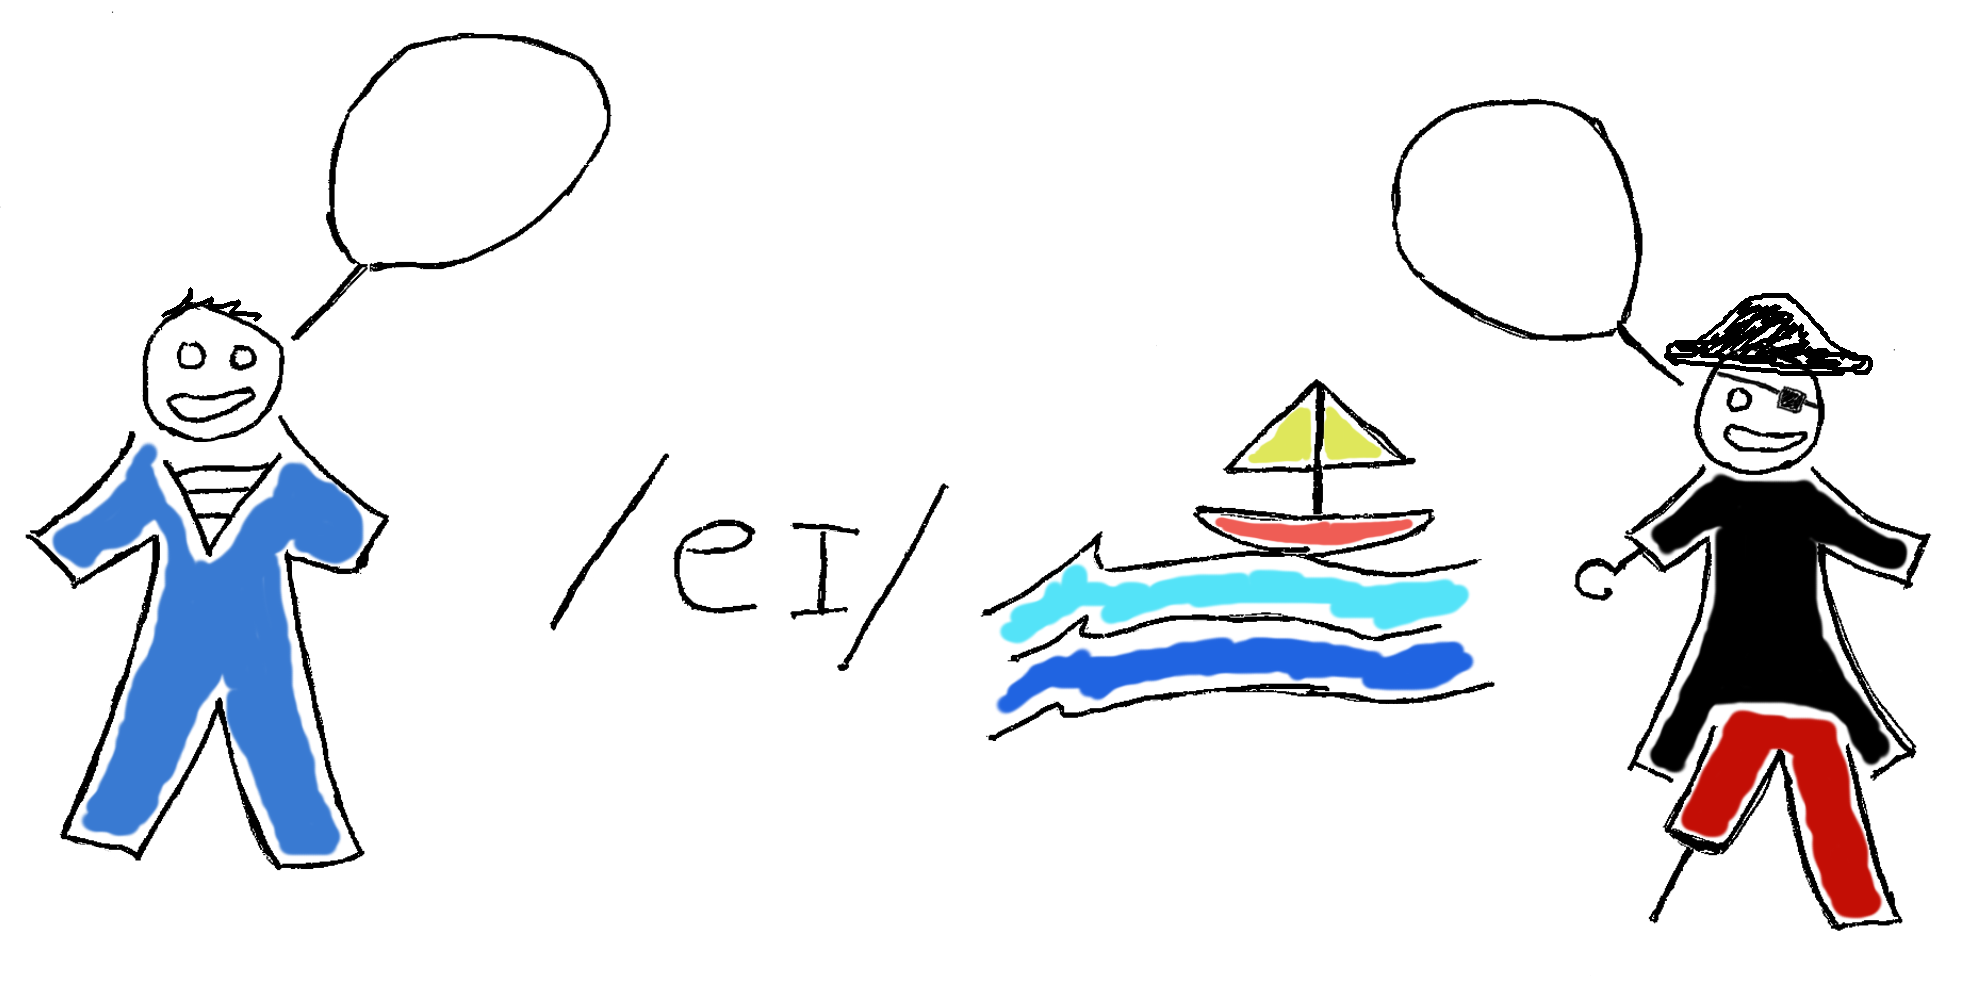
\includegraphics[scale=0.8]{iacr_coloured.png}
\end{turn}
\end{center}
\caption{A new flag for the IACR.\label{fig:iacr_flag}}
\end{figure}


\newcommand{\mybibtitle}[1]{\textsf{#1.}\hfil}
\newcommand{\mybibauth}[1]{#1.}
\newcommand{\mybibconf}[1]{\hspace*{\stretch{1}}\mbox{(#1)}}
\newcolumntype{z}{p{5em}}

\setcounter{section}{0}
\renewcommand\thesection{\Alph{section}}
\section[Mes publications]{My publications}

\subsection{Article de journal}

\noindent
\begin{tabularx}{\linewidth}{zX}
  \cite{asasajour} &
  \mybibtitle{Key-Recovery Attacks on ASASA}
  \mybibauth{B.~Minaud, P.~Derbez, P.-A.~Fouque, P.~Karpman}
  \mybibconf{Invité au J. Cryptology} \\
\end{tabularx}

\subsection{Articles de conférences}

\noindent
\begin{tabularx}{\linewidth}{zX}
  \cite{puppycipher} &
  \mybibtitle{Efficient and Provable White-Box Primitives}
  \mybibauth{P.-A.~Fouque, P.~Karpman, P.~Kirchner, B.~Minaud}
  \mybibconf{ASIACRYPT 2016} \\[2ex]
  \cite{DBLP:conf/eurocrypt/StevensKP16} &
  \mybibtitle{Freestart Collision for Full SHA-1}
  \mybibauth{M.~Stevens, P.~Karpman, T.~Peyrin}
  \mybibconf{EUROCRYPT 2016} \\[2ex]
  \cite{DBLP:conf/asiacrypt/MinaudDFK15} &
  \mybibtitle{Key-Recovery Attacks on ASASA}
  \mybibauth{B.~Minaud, P.~Derbez, P.-A.~Fouque, P.~Karpman}
  \mybibconf{ASIACRYPT 2015} \\[2ex]
  \cite{DBLP:conf/isw/Karpman15} &
  \mybibtitle{From Distinguishers to Key Recovery: Improved Related-Key Attacks on Even-Mansour}
  \mybibauth{P.~Karpman}
  \mybibconf{ISC 2015} \\[2ex]
  \cite{DBLP:conf/crypto/KarpmanPS15} &
  \mybibtitle{Practical Free-Start Collision Attacks on 76-step SHA-1}
  \mybibauth{P.~Karpman, T.~Peyrin, M.~Stevens}
  \mybibconf{CRYPTO 2015} \\[2ex]
  \cite{DBLP:conf/crypto/EspitauFK15} &
  \mybibtitle{Higher-Order Differential Meet-in-the-middle Preimage Attacks on SHA-1 and BLAKE}
  \mybibauth{T.~Espitau, P.-A.~Fouque, P.~Karpman}
  \mybibconf{CRYPTO 2015} \\[2ex]
  \cite{DBLP:conf/sacrypt/AugotFK14} &
  \mybibtitle{Diffusion Matrice from Algebraic-Geometry Codes with Efficient SIMD Implementation}
  \mybibauth{D.~Augot, P.-A.~Fouque, P.~Karpman}
  \mybibconf{SAC 2014} \\[2ex]
  \cite{DBLP:conf/ctrsa/0001KNWW14} &
  \mybibtitle{Analysis of BLAKE2}
  \mybibauth{J.~Guo, P.~Karpman, I. Nikolić, L. Wang, S. Wu}
  \mybibconf{CT-RSA 2014} \\[2ex]
  \cite{DBLP:conf/ima/FouqueK13} &
  \mybibtitle{Security Amplification against Meet-in-the-Middle Attacks Using Whitening}
  \mybibauth{P.-A.~Fouque, P.~Karpman}
  \mybibconf{IMACC 2013} \\
\end{tabularx}

\subsection{Prépublication}

\noindent
\begin{tabularx}{\linewidth}{zX}
  \cite{fly} &
  \mybibtitle{The \textsc{Littlun} S-box and the \textsc{Fly} block cipher}
  \mybibauth{P.~Karpman, B.~Grégoire}\\
\end{tabularx}

\section[Mes publications humoristiques]{My silly talks}

\subsection{Article de journal}

\noindent
\begin{tabularx}{\linewidth}{zX}
  & \mybibtitle{A new flag for the IACR}
  \mybibauth{P.~Karpman}
  \mybibconf{Invité au J. Craptology}\\
\end{tabularx}

\subsection{Présentations sans actes}

\noindent
\begin{tabularx}{\linewidth}{zX}
  &
  \mybibtitle{The Coffee Block Cipher Family --- A Snake Oil Candidate}
  \mybibauth{P.~Karpman}
  \mybibconf{ASIACRYPT 2014 (Rump session)}\\[2ex]
  &
  \mybibtitle{The \emph{Real} SHA-2,3,$\ldots$}
  \mybibauth{P.~Karpman}
  \mybibconf{CRYPTO 2015 (Rump session)}\\[2ex]
  &
  \mybibtitle{Breaking D.L. at Mont Saint-Michel}
  \mybibauth{P.~Karpman, B.~Minaud, A.~Wallet}
  \mybibconf{CHES 2015 (Rump session)}\\[2ex]
  &
  \mybibtitle{A new flag for the IACR}
  \mybibauth{P.~Karpman}
  \mybibconf{ASIACRYPT 2015 (Rump session)}\\
\end{tabularx}


\renewcommand\thesection{\arabic{section}}
